% Options for packages loaded elsewhere
\PassOptionsToPackage{unicode}{hyperref}
\PassOptionsToPackage{hyphens}{url}
%
\documentclass[
  ignorenonframetext,
]{beamer}
\usepackage{pgfpages}
\setbeamertemplate{caption}[numbered]
\setbeamertemplate{caption label separator}{: }
\setbeamercolor{caption name}{fg=normal text.fg}
\beamertemplatenavigationsymbolsempty
% Prevent slide breaks in the middle of a paragraph
\widowpenalties 1 10000
\raggedbottom
\setbeamertemplate{part page}{
  \centering
  \begin{beamercolorbox}[sep=16pt,center]{part title}
    \usebeamerfont{part title}\insertpart\par
  \end{beamercolorbox}
}
\setbeamertemplate{section page}{
  \centering
  \begin{beamercolorbox}[sep=12pt,center]{part title}
    \usebeamerfont{section title}\insertsection\par
  \end{beamercolorbox}
}
\setbeamertemplate{subsection page}{
  \centering
  \begin{beamercolorbox}[sep=8pt,center]{part title}
    \usebeamerfont{subsection title}\insertsubsection\par
  \end{beamercolorbox}
}
\AtBeginPart{
  \frame{\partpage}
}
\AtBeginSection{
  \ifbibliography
  \else
    \frame{\sectionpage}
  \fi
}
\AtBeginSubsection{
  \frame{\subsectionpage}
}
\usepackage{lmodern}
\usepackage{amssymb,amsmath}
\usepackage{ifxetex,ifluatex}
\ifnum 0\ifxetex 1\fi\ifluatex 1\fi=0 % if pdftex
  \usepackage[T1]{fontenc}
  \usepackage[utf8]{inputenc}
  \usepackage{textcomp} % provide euro and other symbols
\else % if luatex or xetex
  \usepackage{unicode-math}
  \defaultfontfeatures{Scale=MatchLowercase}
  \defaultfontfeatures[\rmfamily]{Ligatures=TeX,Scale=1}
\fi
% Use upquote if available, for straight quotes in verbatim environments
\IfFileExists{upquote.sty}{\usepackage{upquote}}{}
\IfFileExists{microtype.sty}{% use microtype if available
  \usepackage[]{microtype}
  \UseMicrotypeSet[protrusion]{basicmath} % disable protrusion for tt fonts
}{}
\makeatletter
\@ifundefined{KOMAClassName}{% if non-KOMA class
  \IfFileExists{parskip.sty}{%
    \usepackage{parskip}
  }{% else
    \setlength{\parindent}{0pt}
    \setlength{\parskip}{6pt plus 2pt minus 1pt}}
}{% if KOMA class
  \KOMAoptions{parskip=half}}
\makeatother
\usepackage{xcolor}
\IfFileExists{xurl.sty}{\usepackage{xurl}}{} % add URL line breaks if available
\IfFileExists{bookmark.sty}{\usepackage{bookmark}}{\usepackage{hyperref}}
\hypersetup{
  pdftitle={Presentación de la Asignatura Tecnologías para el Análisi de Datos Masivos},
  pdfauthor={Máster de Análisis de Datos Masivos UIB: Juan Gabriel Gomila \& Ricardo Alberich},
  hidelinks,
  pdfcreator={LaTeX via pandoc}}
\urlstyle{same} % disable monospaced font for URLs
\newif\ifbibliography
\setlength{\emergencystretch}{3em} % prevent overfull lines
\providecommand{\tightlist}{%
  \setlength{\itemsep}{0pt}\setlength{\parskip}{0pt}}
\setcounter{secnumdepth}{-\maxdimen} % remove section numbering

\title{Presentación de la Asignatura Tecnologías para el Análisi de
Datos Masivos}
\author{Máster de Análisis de Datos Masivos UIB: Juan Gabriel Gomila \&
Ricardo Alberich}
\date{17/10/2020}

\begin{document}
\frame{\titlepage}

\begin{frame}{¿Quiénes somos?}
\protect\hypertarget{quiuxe9nes-somos}{}
\begin{figure}
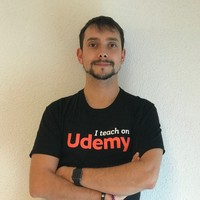
\includegraphics[width=0.25\linewidth]{joanby} \caption{Juan Gabriel Gomila}\label{fig:foto_jb}
\end{figure}

\begin{figure}
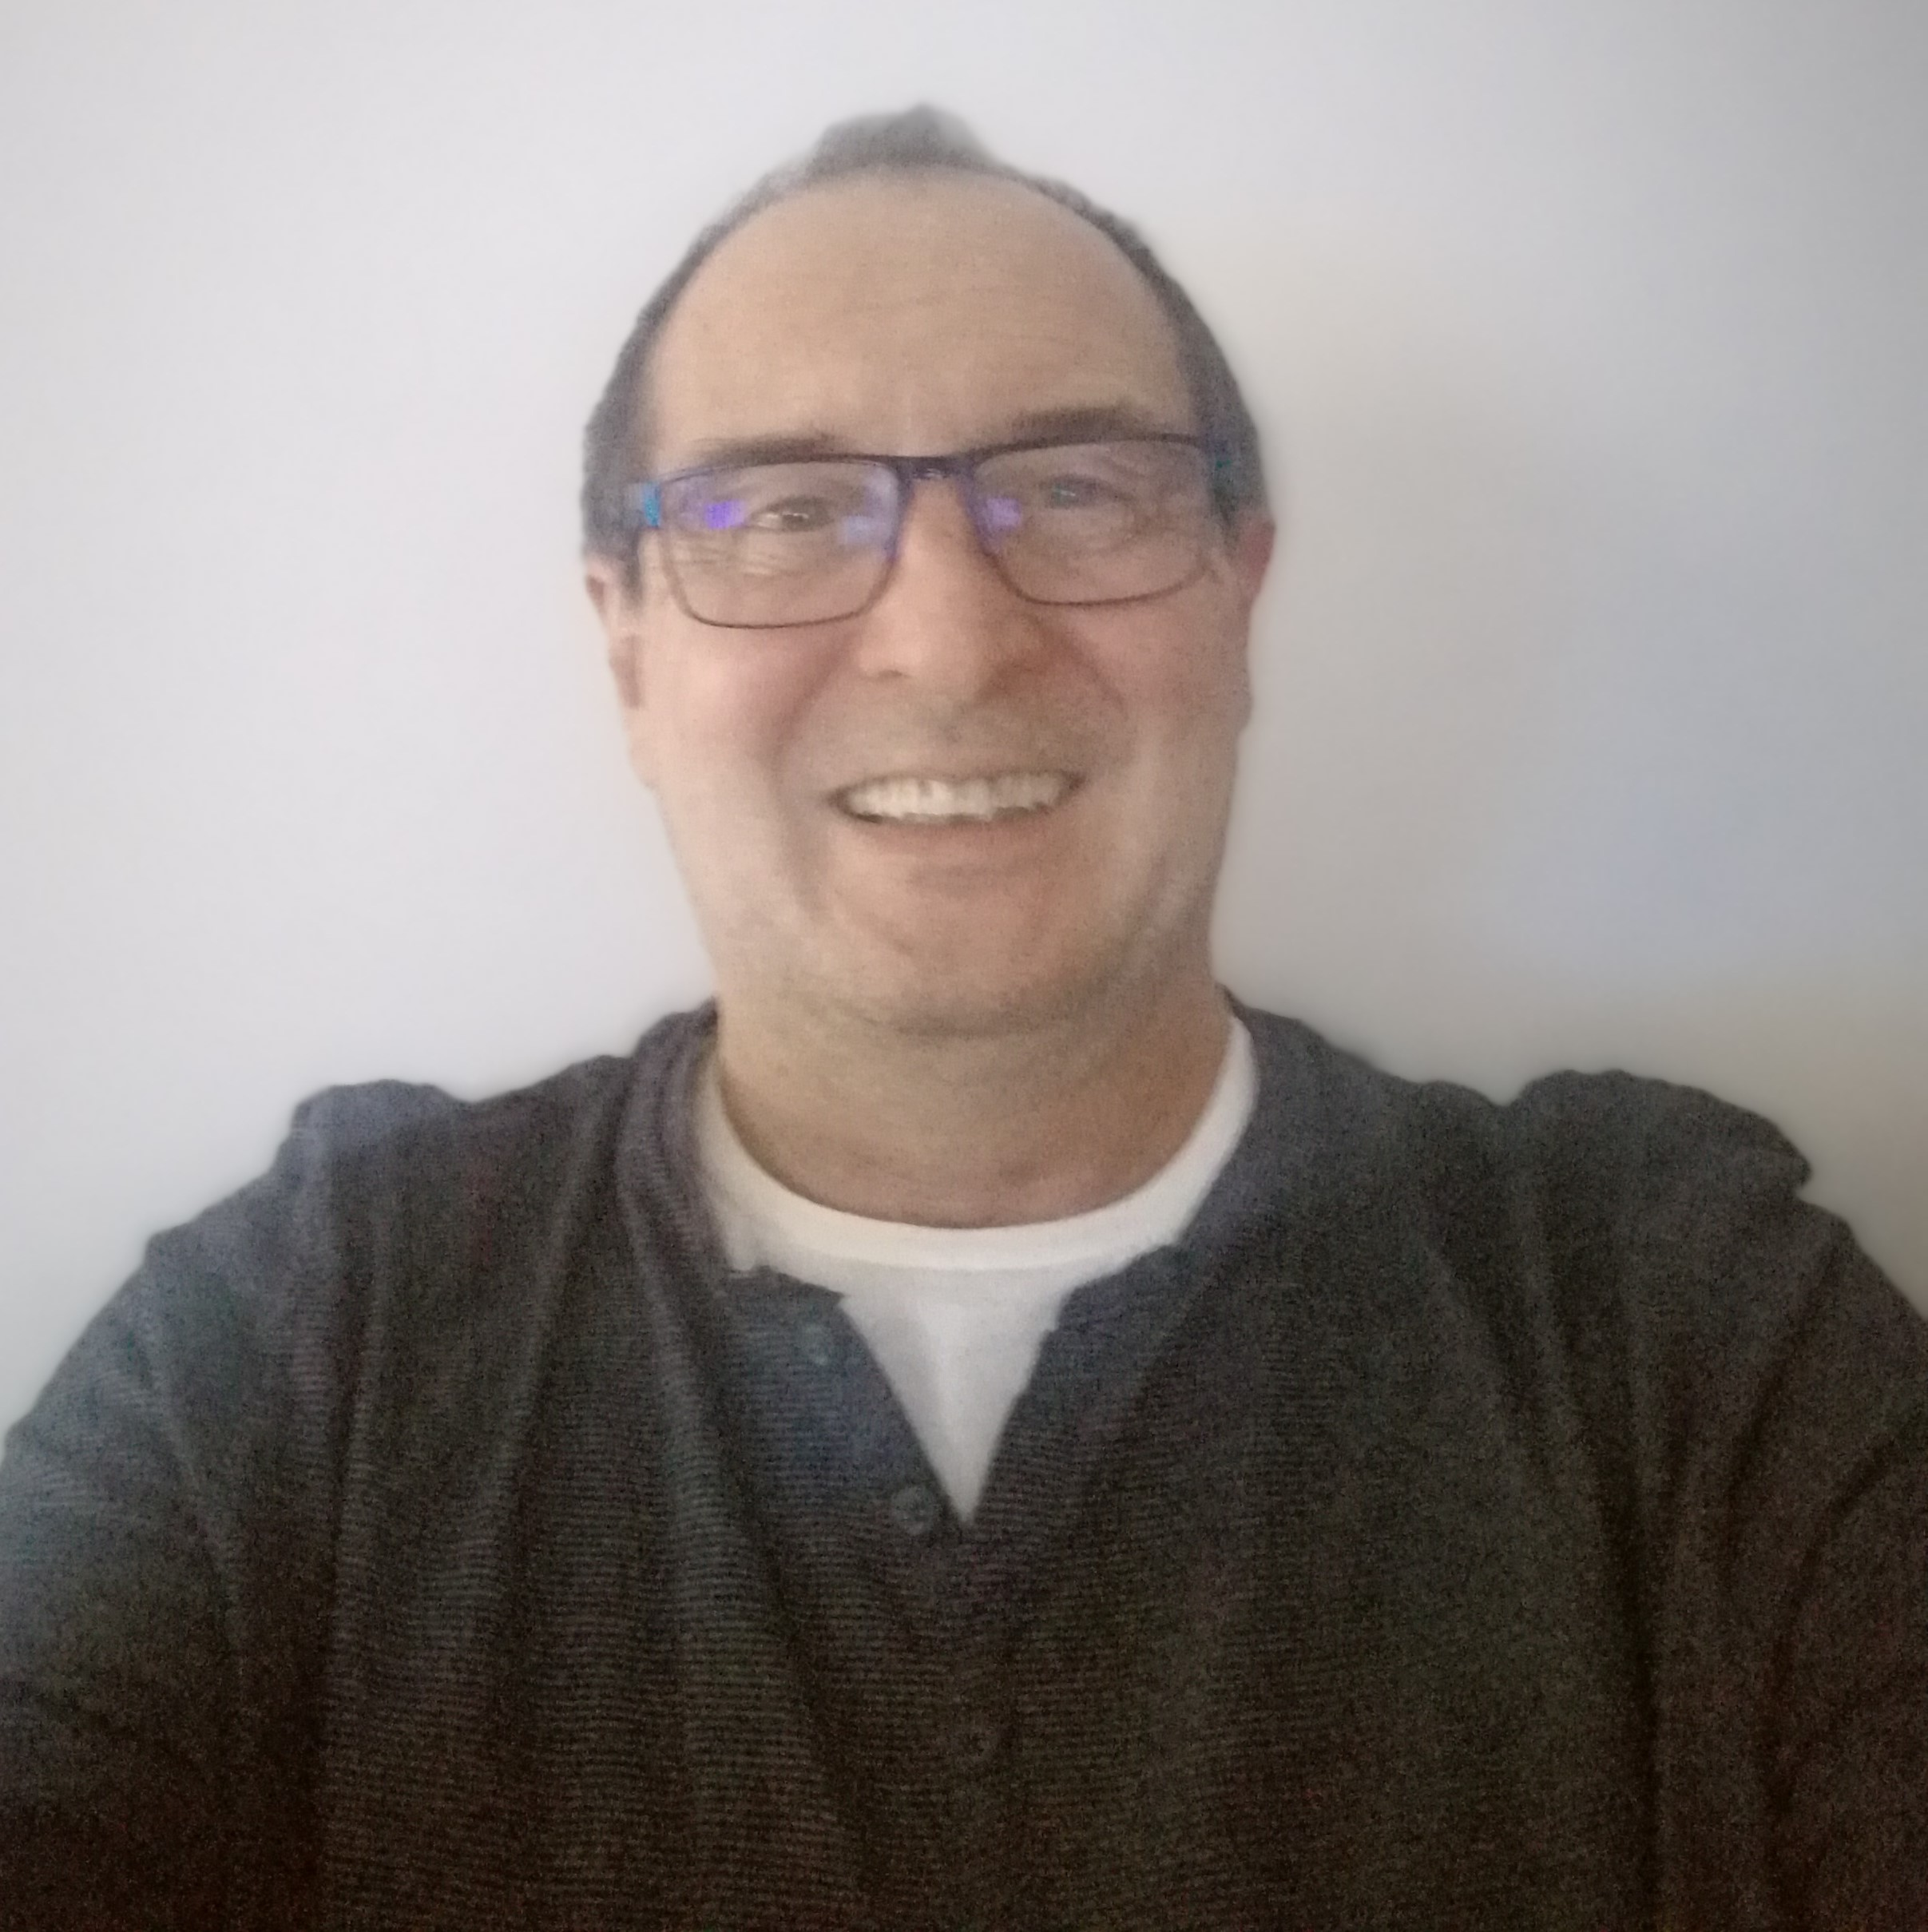
\includegraphics[width=0.25\linewidth]{ra_2020_2} \caption{Ricardo Alberich}\label{fig:foto_ra}
\end{figure}
\end{frame}

\begin{frame}{¿Quiénes somos? Juan Gabriel Gomila}
\protect\hypertarget{quiuxe9nes-somos-juan-gabriel-gomila}{}
\begin{itemize}
\tightlist
\item
  \href{https://www.uib.es/es/lauib/Govern-i-organitzacio/estructura/Departaments/dmi/}{Departamento
  de Ciencias Matemáticas e Informática e la UIB}
\item
  \href{https://www.uib.eu/personal/ABjE5ODE5MA/}{Profesor asociado del
  área de Ciencia de la Computación e Inteligencia artificial}
\item
  \href{https://www.uib.es/es/}{Licenciado en Matemáticas por la UIB}
\item
  \href{https://frogames.es/}{CEO Frogames}
\item
  Y más cosas\ldots{}
\item
  \href{mailto:juan.gabriel.gomila@uib.es}{Email}
\end{itemize}
\end{frame}

\begin{frame}{¿Quiénes somos? Ricardo Alberich}
\protect\hypertarget{quiuxe9nes-somos-ricardo-alberich}{}
\begin{itemize}
\tightlist
\item
  \href{https://www.uib.es/es/lauib/Govern-i-organitzacio/estructura/Departaments/dmi/}{Departamento
  de Ciencias Matemáticas e Informática e la UIB}
\item
  \href{https://www.uib.es/es/personal/ABDI0ODk/}{Profesor Titular del
  área de Ciencia de la Computación e Inteligencia Artificial}
\item
  \href{https://www.uv.es/uvweb/universidad/es/universidad-valencia-1285845048380.html}{Licenciado
  en matemáticas por la Universidad de Valencia}
\item
  \href{https://www.uib.cat/}{Doctor en informática por la UIB}
\item
  \href{mailto:r.alberich@uib.es}{Email}
\end{itemize}
\end{frame}

\begin{frame}{Asignatura 11630 - Tecnologías para el Analisis de Datos
Masivos}
\protect\hypertarget{asignatura-11630---tecnologuxedas-para-el-analisis-de-datos-masivos}{}
\begin{itemize}
\tightlist
\item
  \href{https://academic.uib.es/doa/consultaPublica/look\%5bconpub\%5dMostrarPubGuiaDocAs?entradaPublica=true\&idiomaPais=ca.ES\&_anoAcademico=2020\&_codAsignatura=11630}{Guía
  docente(català)}
\item
  \href{https://academic.uib.es/pds/consultaPublica/look\%5Bconpub\%5DInicioPubHora?entradaPublica=true\&lock=true\&idiomaPais=es.ES\&planDocente=2020\&centro=9395\&estudio=260\&planEstudio=590\&curso=1\&trimestre=S/1\&asignatura11630=11630\&\&grupo0=1\&consultarAsignaturaGrupoPrivada=S}{Cronograma:
  Horarios de clase}
\item
  \href{https://discord.gg/uphEZMR}{Espacio discord de la asignatura}
\item
  \href{https://ad.uib.es/estudis2021/course/view.php?id=1524}{Espacio
  moodle de la UIB de la asignatura}
\end{itemize}
\end{frame}

\begin{frame}{Contenidos de la asignatura y 1}
\protect\hypertarget{contenidos-de-la-asignatura-y-1}{}
Todo será de carácter práctico y aplicado. Ya se profundizará en otras
asignaturas según los itinerarios que hayáis elegido.

Grandes temas (no necesariamente en este orden) son tecnologías para:

\begin{itemize}
\tightlist
\item
  Parte 1 - Preprocesamiento de datos
\item
  Parte 2 - Regresión: Regresión Lineal Simple, Regresión Lineal
  Múltiple, Regresión Polinomial, SVR, Regresión en Árboles de Decisión
  y Regresión con Bosques Aleatorios
\item
  Parte 3 - Clasificación: Regresión Logística, K-NN, SVM, Kernel SVM,
  Naive Bayes, Clasificación con Árboles de Decisión y Clasificación con
  Bosques Aleatorios
\item
  Parte 4 - Clustering: K-Means, Clustering Jerárquico
\item
  Parte 5 - Aprendizaje por Reglas de Asociación: Apriori, Eclat
\end{itemize}
\end{frame}

\begin{frame}{Contenidos de la asignatura y 2}
\protect\hypertarget{contenidos-de-la-asignatura-y-2}{}
Continuación

\begin{itemize}
\tightlist
\item
  Parte 6 - Reinforcement Learning: Límite de Confianza Superior,
  Muestreo Thompson
\item
  Parte 7 - Procesamiento Natural del Lenguaje: Modelo de Bag-of-words y
  algoritmos de NLP
\item
  Parte 8 - Deep Learning: Redes Neuronales Artificiales y Redes
  Neuronales Convolucionales
\item
  Parte 9 - Reducción de la dimensión: ACP, LDA, Kernel ACP
\item
  Parte 10 - Selección de Modelos \& Boosting: k-fold Cross Validation,
  Ajuste de Parámetros, Grid Search, XGBoost
\end{itemize}
\end{frame}

\end{document}
